%\documentclass[12pt,a4paper,oneside]{reportu}
\documentclass[letterpaper, oneside, 12pt, these, creativecommons]{thETS}
\usepackage{times}
\usepackage[pdftex]{graphicx}
\usepackage{multirow}
\usepackage{pdfpages}
\usepackage{amsmath}
\usepackage{amssymb}
\usepackage{caption}
\usepackage[utf8]{inputenc}
\usepackage[frenchb]{babel}
\usepackage{amsmath}
\usepackage{caption}
\usepackage{multibib}
\usepackage{url}
\urlstyle{rm}

\begin{document}

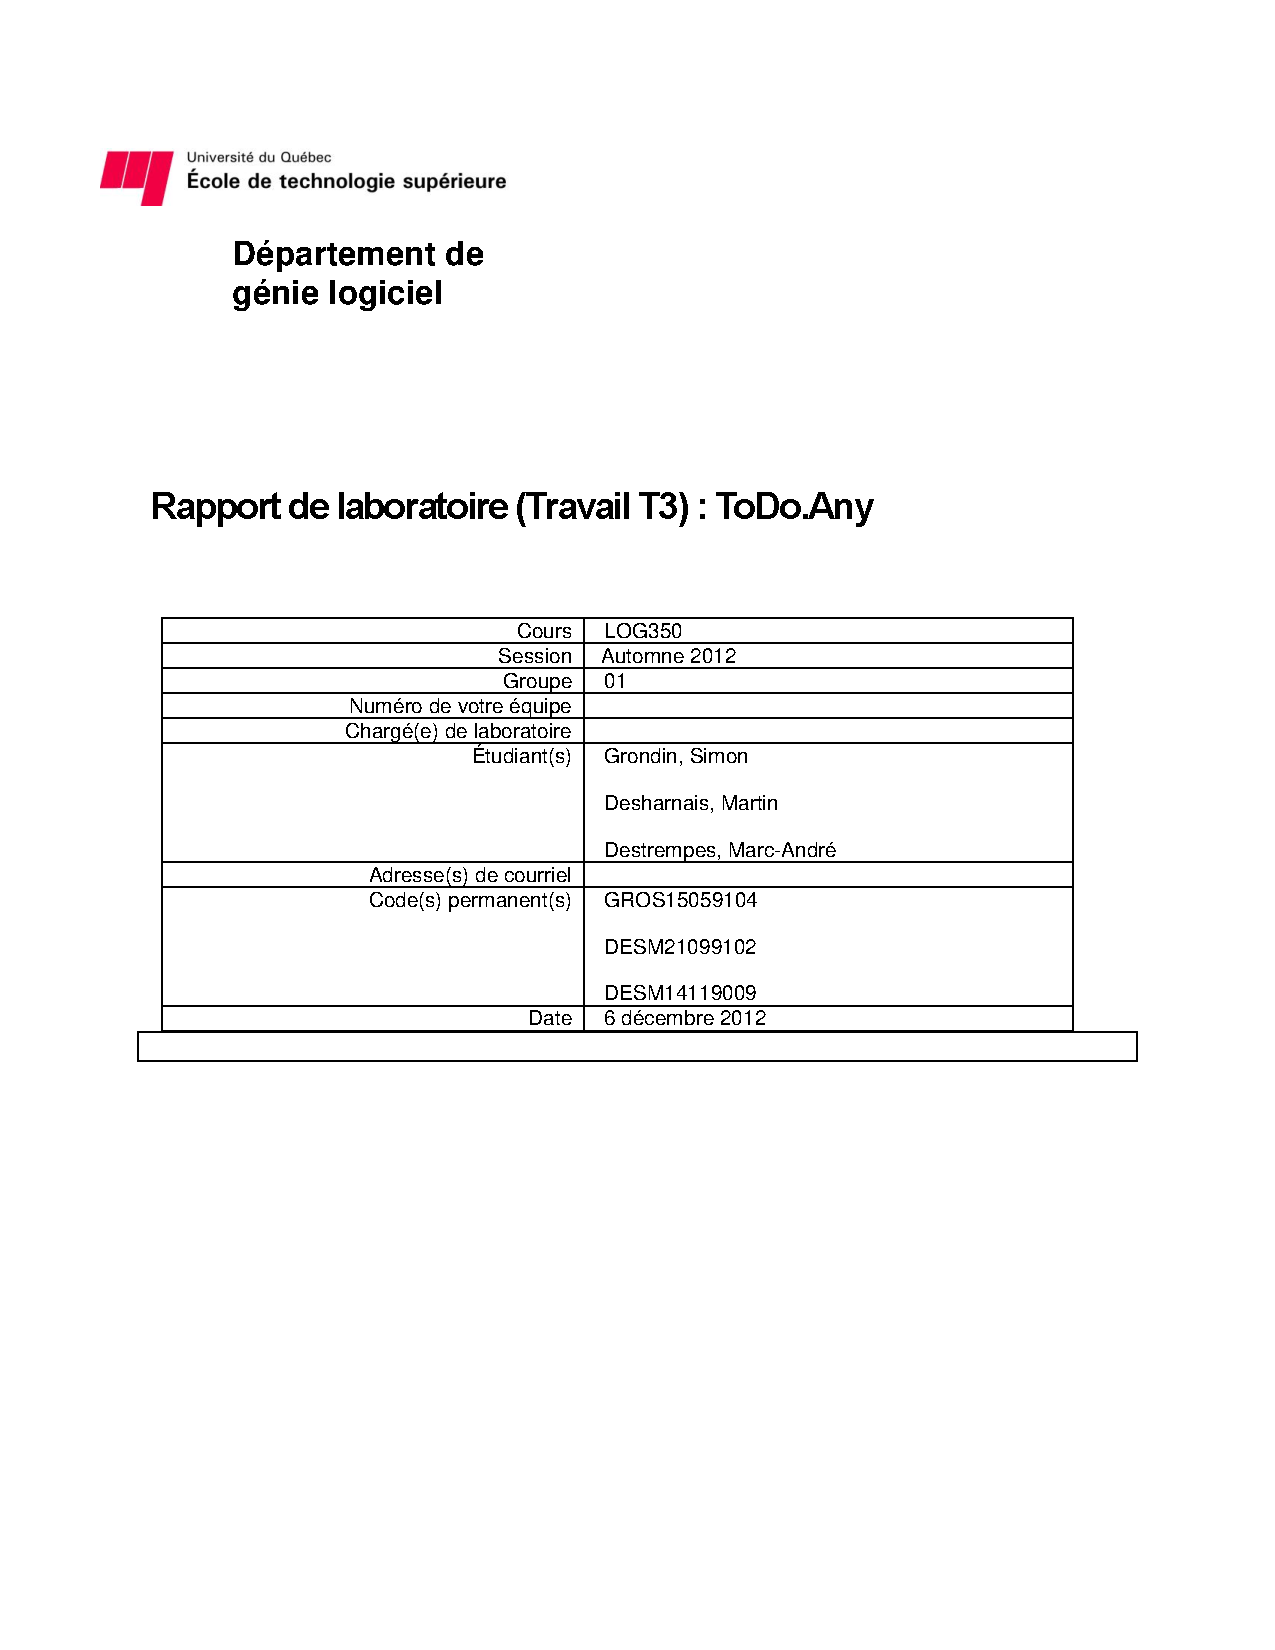
\includepdf[pages=-]{pageTitre.pdf}

\tableofcontents
\listoftables
\listoffigures

\chapter{Introduction et sommaire du travail effectue en TP2}

L'application permet la gestion simple de taches et d'evenements tout en offrant des fonctionnalites de gestion et de classification avancees. Parmi celles-ci, notons la possibilite de definir des rappels, de categoriser les elements, de definir un evenement comme echeance d'une tache ou encore de definir des sous-taches a une tache imposante.

Durant notre analyse de tache, nous avons determiner que le publique cible est des personnes de 15 ans et plus desirant organiser son temps et sa vie professionnelle. De plus, nous avons conclu que notre interface devrais ressembler a des interfaces connu pour la garder familiere et garder une courbe d'apprentissage faible. Pour ce faire, nous avons dresser une liste des cas d'utilisation que l'application doit traiter pour se donner un point de depart. Par la suite, nous avons construit nos prototypes statiques.

Pour construire notre prototype statique, nosu avons utiliser des fenetres virtuelles ou chaques points de chaque fenetre a ete detaille pour s'assurer que le travail devant etre effectue par chaque interface a bel et bien ete compris. De plus, chaque fonctionnalite a aussi ete detaille dans le but qu'elles soient bien comprise.

Jusqu'a present, aucune modification n'a ete apporte entre les prototypes statiques et dynamiques. Tout va rester comme indique dans le document precedent.

Dans le present document, les tests qui seront effectue avec des utilisateurs seront listes et detailles. Par la suite, un concensus sera fais pour chaque tache et une amelioration qui pourrait etre faite sera proposer pour ameliorer le comportement du logiciel.

\chapter{Planification du travail}

\begin{table}
	\centering
	\begin{tabular}{|l|l|}
		\hline
		Semaine	& Travail accomplis 								\\ \hline
		4 novembre	& Choix de la technologie et apprentissage de celle-ci.		\\ \hline
		11 novembre	& Marc-André : Conception des interfaces. 				\\
				& Martin : Conception de la base de données.				\\
				& Simon : Conception de la base de données.				\\ \hline
		18 novembre	& Marc-André : Début de la rédaction du rapport. 			\\ 
				& Martin : Programmation du prototype dynamique. 			\\
				& Simon : Programmation du prototype dynamique. 			\\ \hline
		25 novembre	& Marc-André : Rédaction du rapport.		 			\\
				& Martin : Programmation du prototype dynamique. 			\\ 
				& Simon : Programmation du prototype dynamique.		 	\\ \hline
		2 decembre	& Marc-André : Rencontre avec les utilisateurs. 			\\
				& Martin : Rédaction du rapport.						\\
				& Simon : Rédaction du rapport.						\\ \hline
		9 decembre	& Marc-André : Préparation de la présentation.	 		\\ 
				& Martin : Préparation de la présentation.	 			\\ 
				& Simon : Préparation de la présentation.	 			\\ \hline
	\end{tabular}
	\caption{Echéancier}
\end{table}

\chapter{Realisation du prototype dynamique}

\section{Justification des choix de conception}

Divers patrons de conception ont ete utilise pour parvenir a la conception de l'application que nous avons presentement. 

Parmi les divers patrons disponibles, on compte le patron \emph{Many Workspaces} qui se retrouve a la fenetre principale de l'application ou l'utilisateur a la possibilite d'avoir plusieurs listes d'ouvertes et de les organiser comme il veut via des onglets. L'utilisateur peut donc gerer plusieurs listes a la fois. 

Pour la navigation entre les fenetres de l'application nous utilisons le patron \emph{Escape Hatch}. Ainsi, la navigation entre les fenetres est limite et l'utilisateur peut toujours revenir a la fenetre principale sans chercher pendant de longues minutes comment y revenir. Cela simplifie grandement l'interaction entre l'application et l'utilisateur en simplifiant le processus de navigation au maximum. 

Ensuite, pour ce qui est des listes, nous utilisons le patron \emph{Tree Table} sur, par exemple, la fenetre principale. Avec ce patron, nous listons donc les taches et chaque sous-tache sous sa tache correspondante sous forme d'arborescence. Nous pouvons donc afficher un maximum d'information utile a l'utilisateur lorsque celui-ci le demande. Nous utilisons aussi le patron \emph{New-Item Row} dans la fenetre Priorites pour permettre l'ajout rapide et infini de lignes dans le tableau sans que l'utilisateur n'ait besoin d'appuyer sur quoi que se soit. Pour ce qui est de toutes les grilles, le patron \emph{Sortable Table} s'applique et permet de trier l'information affiche en tout temps pour permettre a l'utilisateur de trouver ce qu'il veut plus rapidement. 

De plus, nous avons respecte le plus possible le contenu de la norme \emph{ISO 9241-120} a \emph{ISO 9241-129}.

\section{Ameliorations possibles}

Quelques ameliorations possibles seraient d'utiliser les lois psychomotrices de Fitts et Miller pour optimiser l'interface. Nous pourrions ainsi optimiser les deplacements que l'utilisateur doit faire avec sa souris pour cliquer sur les boutons et les champs de saisies dans les fenetres. Mais, par faute de temps et de ressources humaines, il nous est donc impossible d'effectuer ces tests.

\chapter{Demonstration du prototype dynamique en laboratoire}

Une demonstration du prototype dynamique sera faite en laboratoire le XX decembre 2012.

Un prototype dynamique de l'application est disponible a l'adresse suivante : 
\url{https://github.com/xeph/LOG350.TP3}.

\chapter{Tests avec utilisateurs}

\section{Methodologie}

\newpage

\section{Liste des taches}

\begin{table}
	\centering
	\begin{tabular}{|l|l|l|}
		\hline
		no Tache	& Titre et description		& Elements que vous voulez verifier et hypotheses 	\\ \hline 
		1		& Ajouter un evenement		&  							\\ 
				& sans alertes.			&							\\ \hline
		2		& Modifier l'evenement creer et	&							\\
				& ajouter une alerte.		&							\\ \hline
		3		& Ajouter le tag ecole		&							\\
				& a l'evenement.			&							\\ \hline
		4		& Creer un evenement et		&							\\
				& ajouter le tag travail.		&							\\ \hline
		5		& Rechercher les evenements	& 							\\
				& par tag.				&							\\ \hline
		6		& Supprimer les evenements	&							\\
				& contenant le tag travail.		&							\\ \hline
		7		& Trouver la fenetre des		&							\\
				& priorites.				& 							\\ \hline
		8		& Ajouter une nouvelle priorite 	&							\\
				& valide.				&							\\ \hline
		9		& Desactiver une priorite ne	&							\\
				& contenant aucun evenement ou &							\\
				& tache associe.			&							\\ \hline
		10		& Ajouter plusieurs taches		&							\\
				& (3-5 environ).			&							\\ \hline
		11		& Prendre une tache et lui		&							\\
				& affecter 2 sous-taches.		&							\\ \hline
		12		& Modifier la completion d'une	&							\\
				& tache non complete.		&							\\ \hline
		13		& Modifier la completion de	&							\\
				& sous-taches pour completer	&							\\ 
				& une tache.				&							\\ \hline
		14		& Supprimer une tache complete.	&							\\ \hline
		15		& Modifier les informations		&							\\
				& d'une tache non complete.	&							\\ \hline
		16		& Rechercher une tache avec la 	&							\\
				& priorite cree precedement.	& 							\\ \hline
	\end{tabular}
	\caption{Liste des taches}
\end{table}

\section{Liste des utilisateurs}

Les caracteristiques principales des utilisateurs choisis sont la gestion de leurs taches pour les travaux et devoirs au CEGEP ou bien a l'universite et la gestion des rendez-vous pour les professionnels. Nous avons choisis ce nombre d'utilisateur, car il nous fallait un petit echantillon oeuvrant dans le meme type de vie que le publique visee mais dans des spheres professionnelles differentes. Il est pertinant d'avoir teste avec ces utilisateurs parce que se sera principalement ce type d'utilisateur qui se servira d'une application comme celle-ci.

\newpage

\section{Resultats}

\begin{table}
	\centering
	\begin{tabular}{|l|l|l|}
	\hline
	no Tache	& Points importants de l'observation	\\ \hline
	1		& 0						\\ \hline
	2		& 0						\\ \hline
	3		& 0						\\ \hline
	4		& 0						\\ \hline
	5		& 0						\\ \hline
	6		& 0						\\ \hline
	7		& 0						\\ \hline
	8		& 0						\\ \hline
	9		& 0						\\ \hline
	10		& 0						\\ \hline
	11		& 0						\\ \hline
	12		& 0						\\ \hline
	13		& 0						\\ \hline
	14		& 0						\\ \hline
	15		& 0						\\ \hline
	16		& 0						\\ \hline
	\end{tabular}
	\caption{Resultats de l'utilisateur 1}
\end{table}

\newpage

\begin{table}
	\centering
	\begin{tabular}{|l|l|l|}
	\hline
	no Tache	& Points importants de l'observation	\\ \hline
	1		& 0						\\ \hline
	2		& 0						\\ \hline
	3		& 0						\\ \hline
	4		& 0						\\ \hline
	5		& 0						\\ \hline
	6		& 0						\\ \hline
	7		& 0						\\ \hline
	8		& 0						\\ \hline
	9		& 0						\\ \hline
	10		& 0						\\ \hline
	11		& 0						\\ \hline
	12		& 0						\\ \hline
	13		& 0						\\ \hline
	14		& 0						\\ \hline
	15		& 0						\\ \hline
	16		& 0						\\ \hline
	\end{tabular}
	\caption{Resultats de l'utilisateur 2}
\end{table}

\newpage

\begin{table}
	\centering
	\begin{tabular}{|l|l|l|}
	\hline
	no Tache	& Points importants de l'observation	\\ \hline
	1		& 0						\\ \hline
	2		& 0						\\ \hline
	3		& 0						\\ \hline
	4		& 0						\\ \hline
	5		& 0						\\ \hline
	6		& 0						\\ \hline
	7		& 0						\\ \hline
	8		& 0						\\ \hline
	9		& 0						\\ \hline
	10		& 0						\\ \hline
	11		& 0						\\ \hline
	12		& 0						\\ \hline
	13		& 0						\\ \hline
	14		& 0						\\ \hline
	15		& 0						\\ \hline
	16		& 0						\\ \hline
	\end{tabular}
	\caption{Resultats de l'utilisateur 3}
\end{table}

\newpage

\section{Discussion et recommandations}

\begin{table}
	\centering
	\begin{tabular}{|l|l|l|}
	\hline
	no Tache	& Resume	& Recommandation 	\\ \hline
	1		& 0		& 0 			\\ \hline
	2		& 0		& 0 			\\ \hline
	3		& 0		& 0 			\\ \hline
	4		& 0		& 0 			\\ \hline
	5		& 0		& 0 			\\ \hline
	6		& 0		& 0 			\\ \hline
	7		& 0		& 0 			\\ \hline
	8		& 0		& 0 			\\ \hline
	9		& 0		& 0 			\\ \hline
	10		& 0		& 0 			\\ \hline
	11		& 0		& 0 			\\ \hline
	12		& 0		& 0 			\\ \hline
	13		& 0		& 0 			\\ \hline
	14		& 0		& 0 			\\ \hline
	15		& 0		& 0 			\\ \hline
	16		& 0		& 0 			\\ \hline
	\end{tabular}
\end{table}

\chapter{Changements recommandes}

\chapter{Conclusion}

\appendix
\multiannexe

\chapter{Formulaire de consentement des utilisateurs}

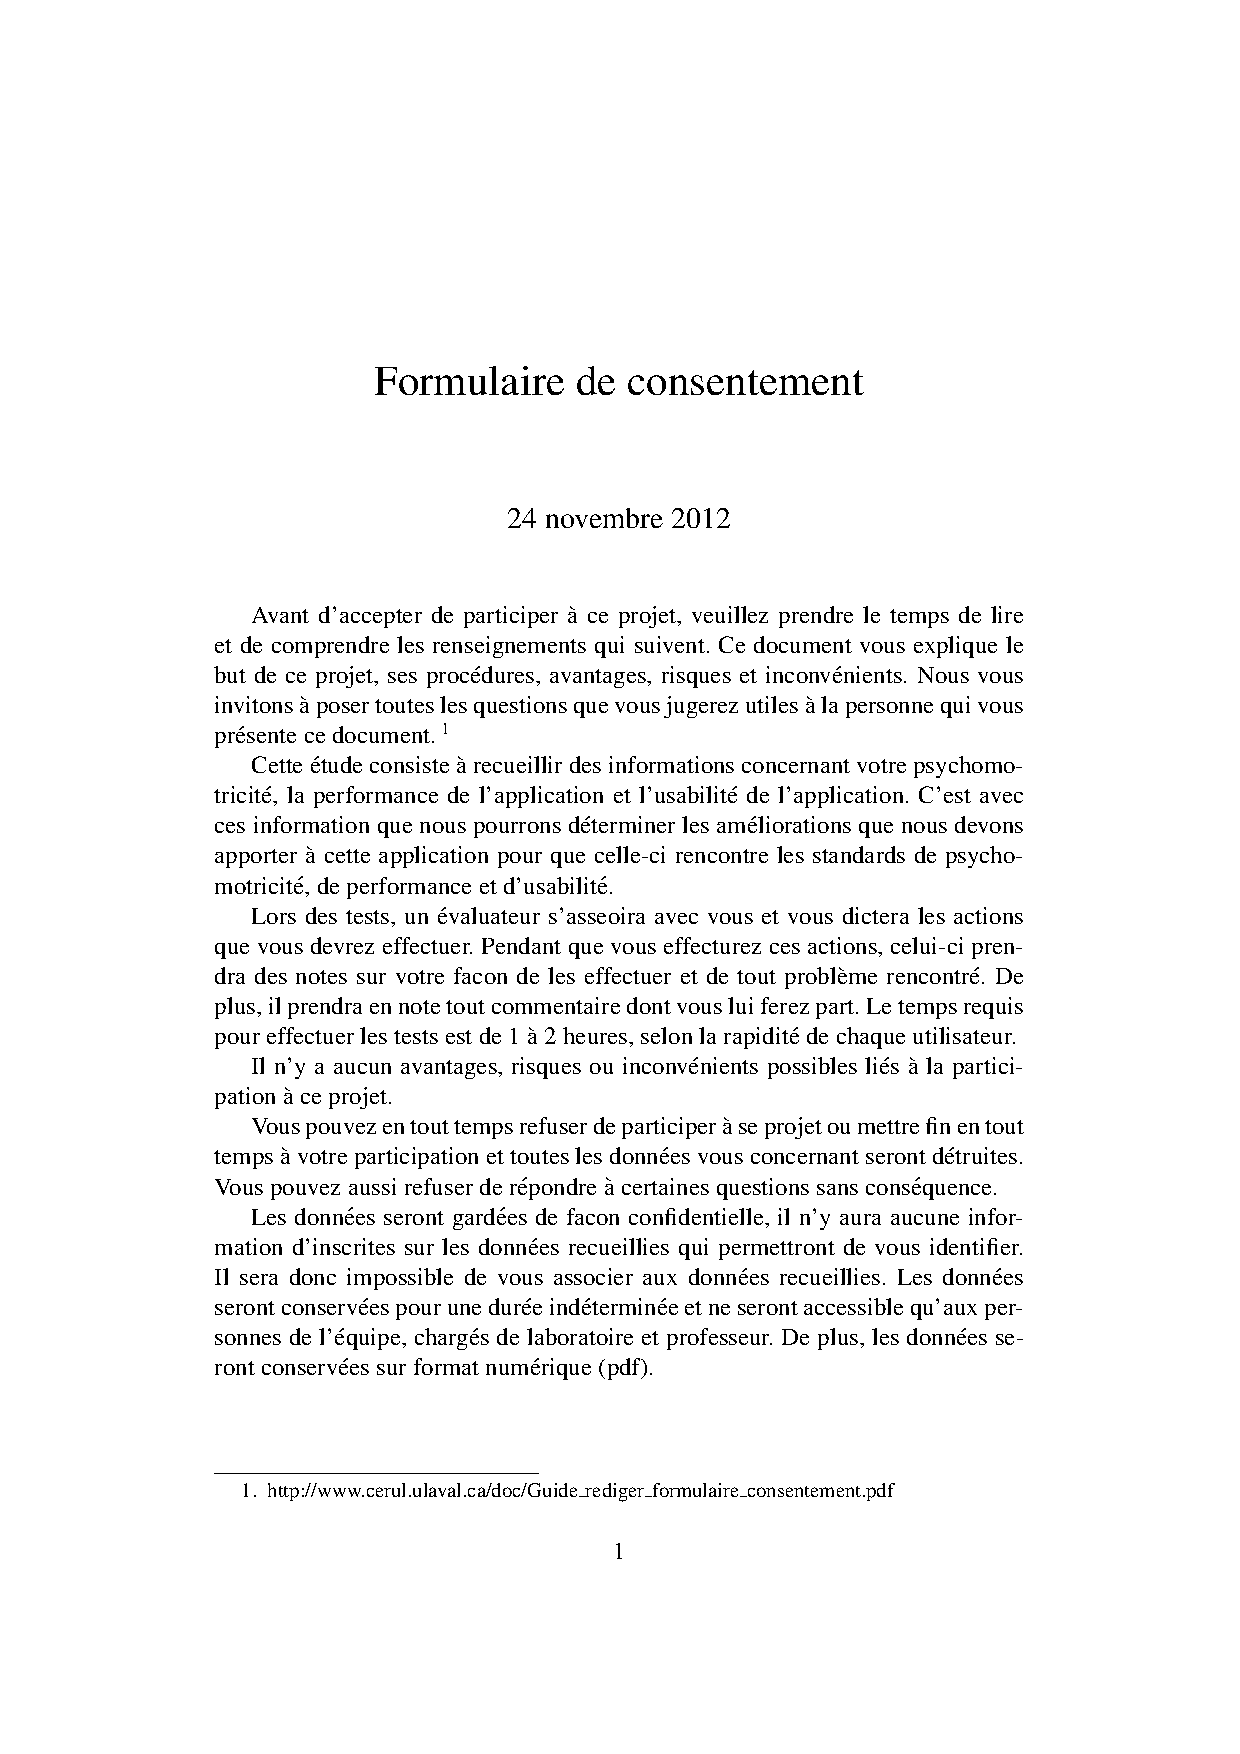
\includepdf[pages=-]{form.pdf}

\chapter{Document de présentation du projet}

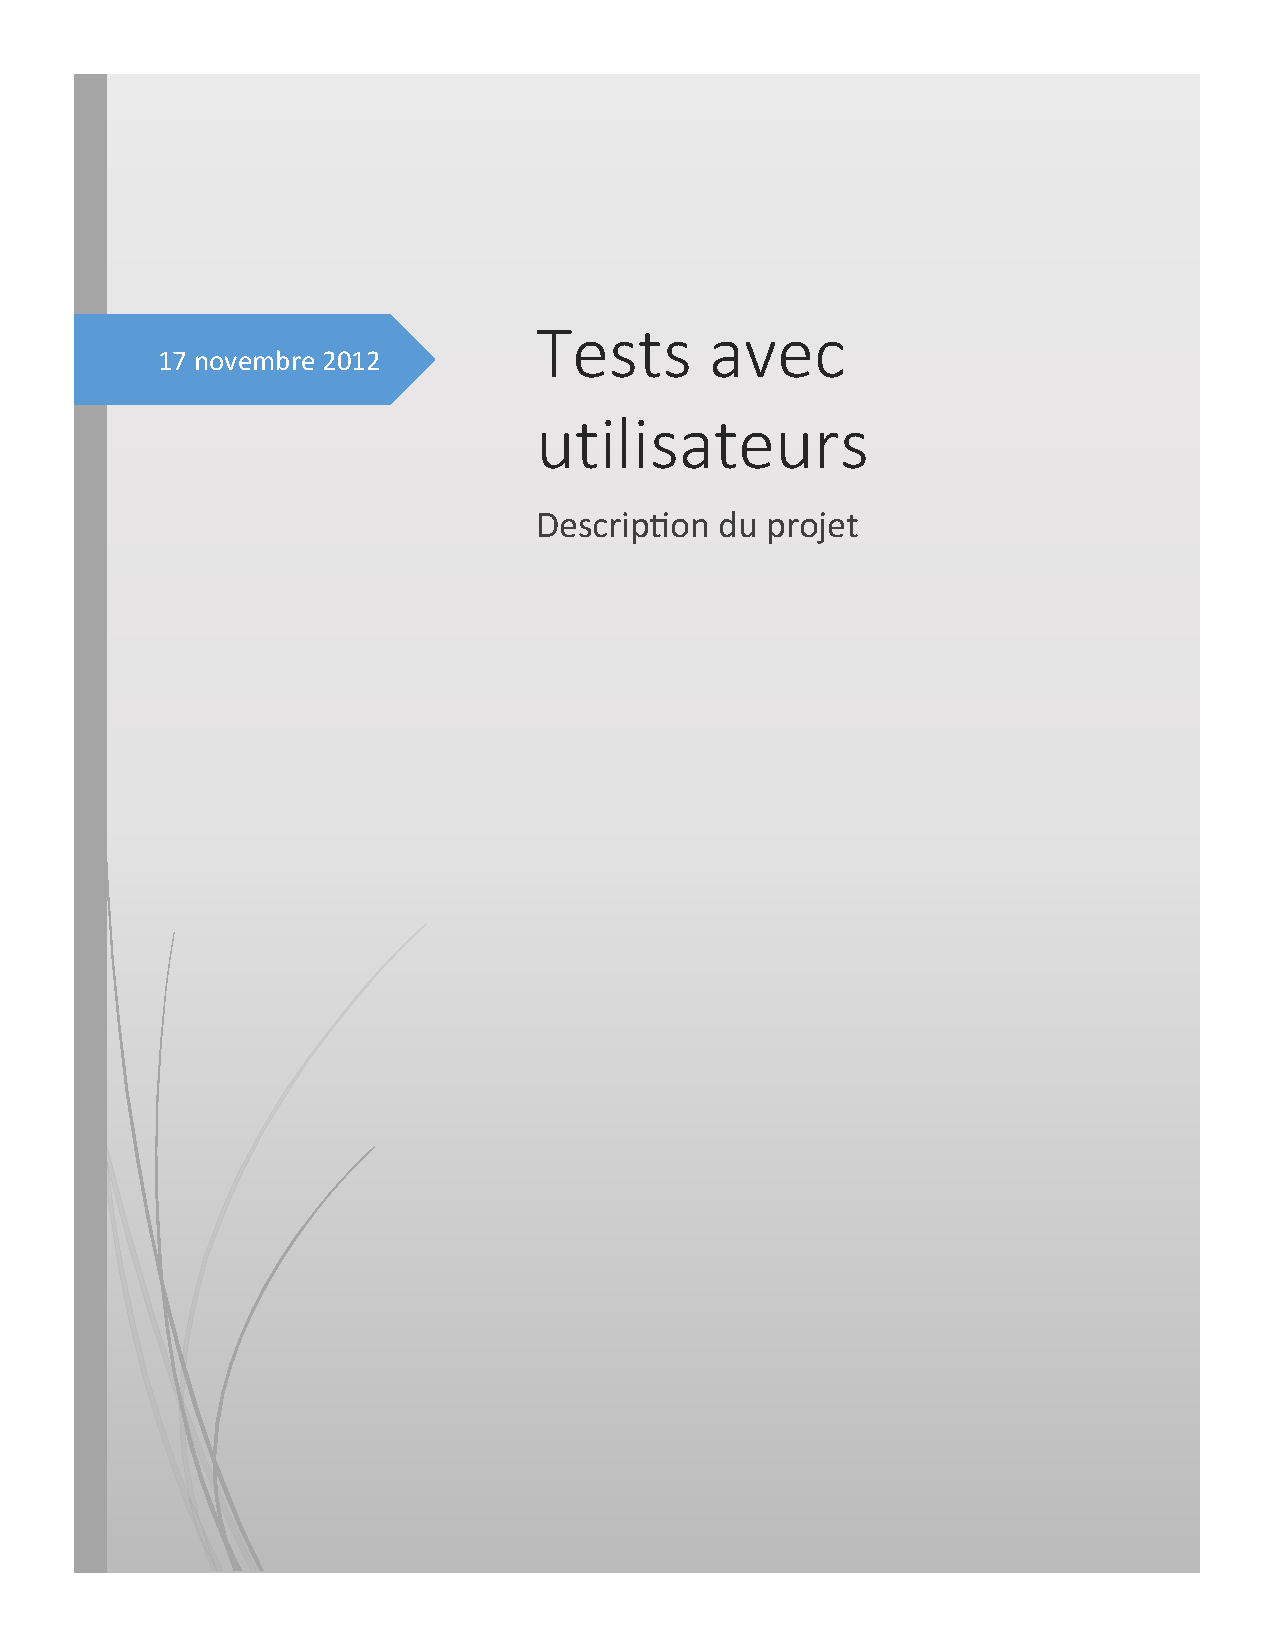
\includepdf[pages=-]{document.pdf}

\chapter{Travail Pratique 2}

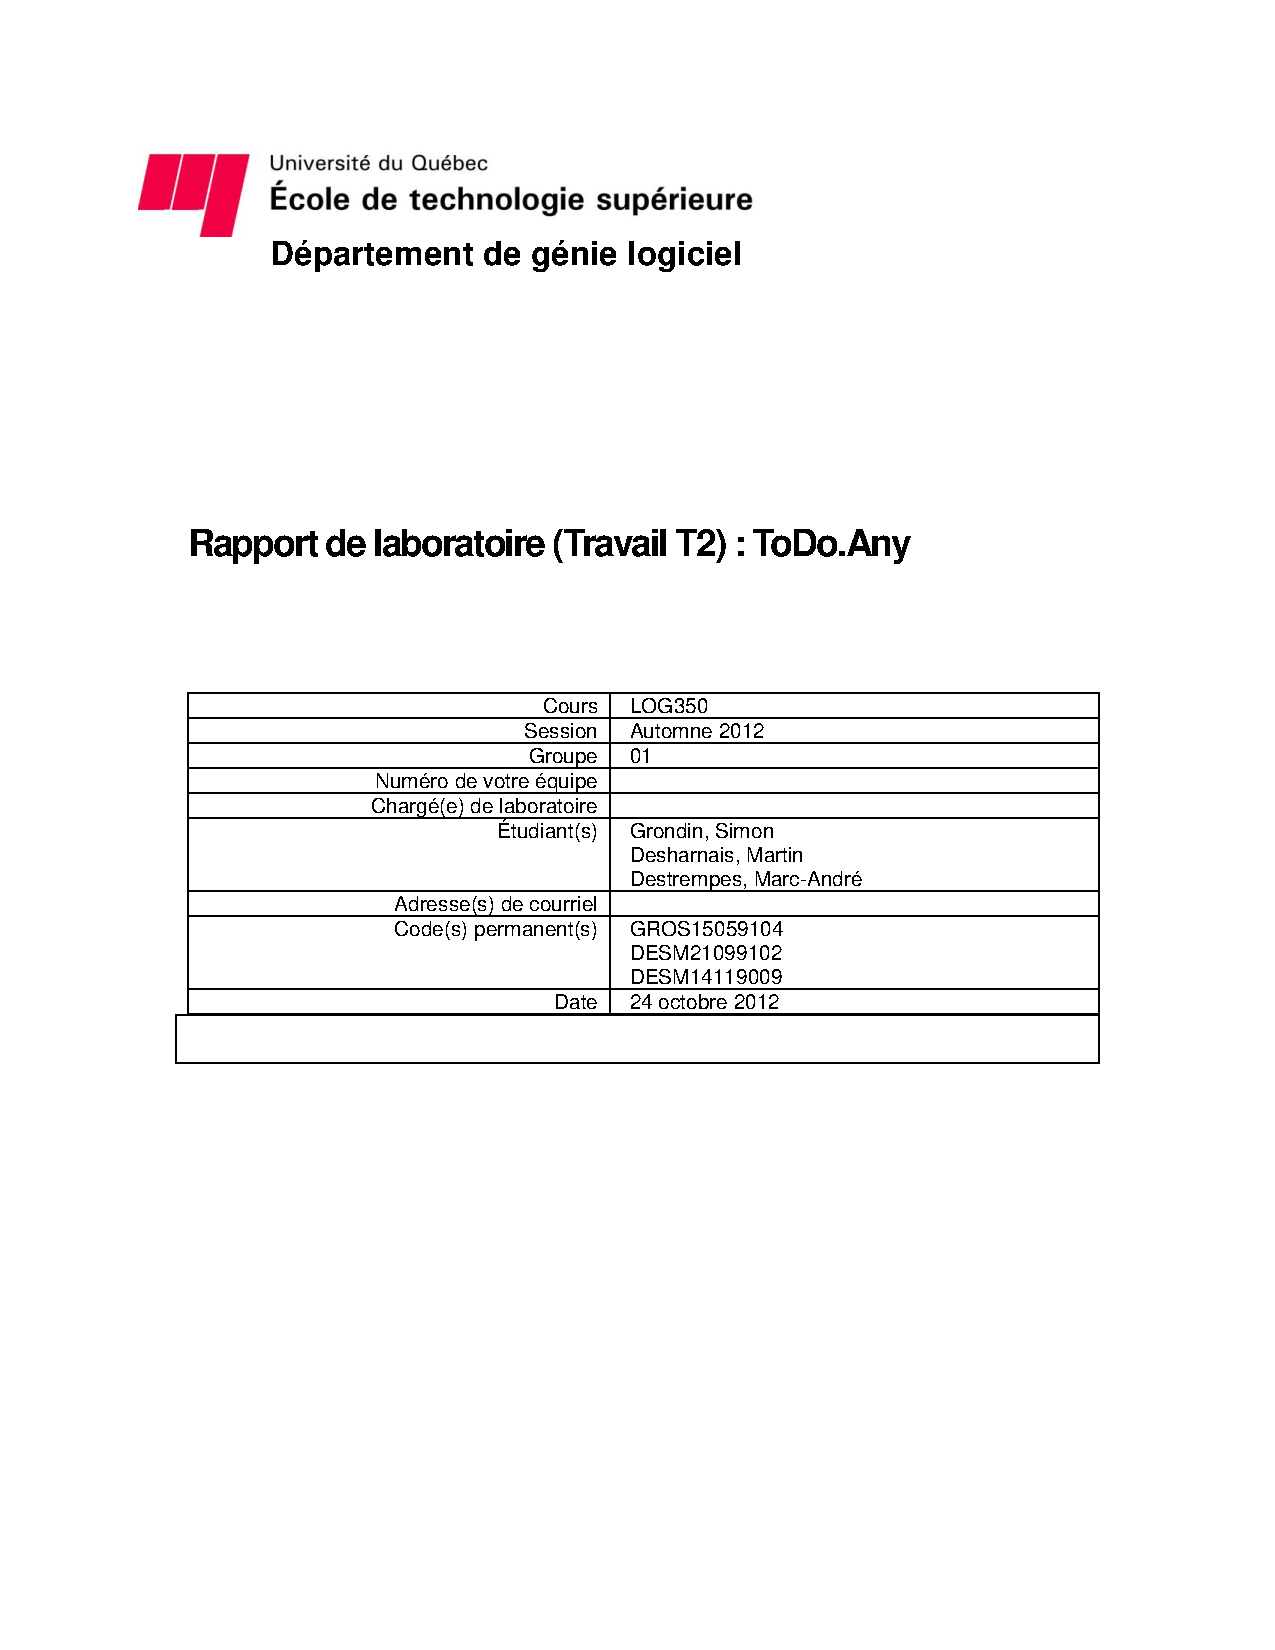
\includepdf[pages=-]{T2.pdf}

\end{document}